\documentclass{sigchi}
% Use this section to set the ACM copyright statement (e.g. for
% preprints).  Consult the conference website for the camera-ready
% copyright statement.
% Copyright
\CopyrightYear{2020}
%\setcopyright{acmcopyright}
\setcopyright{acmlicensed}
%\setcopyright{rightsretained}
%\setcopyright{usgov}
%\setcopyright{usgovmixed}
%\setcopyright{cagov}
%\setcopyright{cagovmixed}
% DOI
\doi{https://doi.org/10.1145/3313831.XXXXXXX}
% ISBN
\isbn{978-1-4503-6708-0/20/04}
%Conference
\conferenceinfo{Asian CHI Symposium '20,}{April  25--30, 2020, Honolulu, HI, USA}
%Price
\acmPrice{\$15.00}
% Use this command to override the default ACM copyright statement
% (e.g. for preprints).  Consult the conference website for the
% camera-ready copyright statement.
%% HOW TO OVERRIDE THE DEFAULT COPYRIGHT STRIP --
%% Please note you need to make sure the copy for your specific
%% license is used here!
% \toappear{
% Permission to make digital or hard copies of all or part of this work
% for personal or classroom use is granted without fee provided that
% copies are not made or distributed for profit or commercial advantage
% and that copies bear this notice and the full citation on the first
% page. Copyrights for components of this work owned by others than ACM
% must be honored. Abstracting with credit is permitted. To copy
% otherwise, or republish, to post on servers or to redistribute to
% lists, requires prior specific permission and/or a fee. Request
% permissions from \href{mailto:Permissions@acm.org}{Permissions@acm.org}. \\
% \emph{CHI '16},  May 07--12, 2016, San Jose, CA, USA \\
% ACM xxx-x-xxxx-xxxx-x/xx/xx\ldots \$15.00 \\
% DOI: \url{http://dx.doi.org/xx.xxxx/xxxxxxx.xxxxxxx}
% }
% Arabic page numbers for submission.  Remove this line to eliminate
% page numbers for the camera ready copy
% \pagenumbering{arabic}
% Load basic packages
\usepackage{balance}    % to better equalize the last page
\usepackage{graphics}   % for EPS, load graphicx instead 
\usepackage[T1]{fontenc}  % for umlauts and other diaeresis
\usepackage{txfonts}
\usepackage{mathptmx}
\usepackage[pdflang={en-US},pdftex,breaklinks]{hyperref}
\usepackage{color}
\usepackage{booktabs}
\usepackage{textcomp}
\usepackage{url}
\def\UrlBreaks{\do\/\do-}
\usepackage{breakurl}
\usepackage{multirow}
\usepackage{dblfloatfix}
\usepackage[super]{nth}

% Some optional stuff you might like/need.
\usepackage{microtype}        % Improved Tracking and Kerning
% \usepackage[all]{hypcap}    % Fixes bug in hyperref caption linking
\usepackage{ccicons}          % Cite your images correctly!
% \usepackage[utf8]{inputenc} % for a UTF8 editor only
% If you want to use todo notes, marginpars etc. during creation of
% your draft document, you have to enable the "chi_draft" option for
% the document class. To do this, change the very first line to:
% "\documentclass[chi_draft]{sigchi}". You can then place todo notes
% by using the "\todo{...}"  command. Make sure to disable the draft
% option again before submitting your final document.
\usepackage{todonotes}
% Paper metadata (use plain text, for PDF inclusion and later
% re-using, if desired).  Use \emtpyauthor when submitting for review
% so you remain anonymous.
\def\plaintitle{Designing Grit: Discovering Features Towards Supporting Novice Programmer DevOps Integration}
\def\plainauthor{Tyrone Justin Sta Maria, Gavin Raine Dizon, Vince Anthony Esquivel, Jordan Aiko Deja and Unisse Chua}
\def\emptyauthor{}
\def\plainkeywords{DevOps; novice programmers; programmer support}
\def\plaingeneralterms{Programming}
% llt: Define a global style for URLs, rather that the default one
\makeatletter
\def\url@leostyle{%
  \@ifundefined{selectfont}{
    \def\UrlFont{\sf}
  }{
    \def\UrlFont{\small\bf\ttfamily}
  }}
\makeatother
\urlstyle{leo}
% To make various LaTeX processors do the right thing with page size.
\def\pprw{8.5in}
\def\pprh{11in}
\special{papersize=\pprw,\pprh}
\setlength{\paperwidth}{\pprw}
\setlength{\paperheight}{\pprh}
\setlength{\pdfpagewidth}{\pprw}
\setlength{\pdfpageheight}{\pprh}
% Make sure hyperref comes last of your loaded packages, to give it a
% fighting chance of not being over-written, since its job is to
% redefine many LaTeX commands.
\definecolor{linkColor}{RGB}{6,125,233}
\hypersetup{%
  pdftitle={\plaintitle},
% Use \plainauthor for final version.
%  pdfauthor={\plainauthor},
  pdfauthor={\emptyauthor},
  pdfkeywords={\plainkeywords},
  pdfdisplaydoctitle=true, % For Accessibility
  bookmarksnumbered,
  pdfstartview={FitH},
  colorlinks,
  citecolor=black,
  filecolor=black,
  linkcolor=black,
  urlcolor=linkColor,
  breaklinks=true,
  hypertexnames=false
}
% create a shortcut to typeset table headings
% \newcommand\tabhead[1]{\small\textbf{#1}}
% End of preamble. Here it comes the document.
\begin{document}
\title{\plaintitle}
\numberofauthors{5}
\author{%
  \alignauthor{Tyrone Justin Sta Maria\\
    \affaddr{De La Salle University}\\
    \affaddr{Manila, Philippines}\\
    \email{tyrone\_stamaria@dlsu.edu.ph}}\\
  \alignauthor{Gavin Raine Dizon\\
    \affaddr{De La Salle University}\\
    \affaddr{Manila, Philippines}\\
    \email{gavin\_dizon@dlsu.edu.ph}}\\
 \alignauthor{Vince Anthony Esquivel\\
    \affaddr{De La Salle University}\\
    \affaddr{Manila, Philippines}\\
    \email{vince\_esquivel@dlsu.edu.ph}}\\
\alignauthor{Jordan Aiko Deja\thanks{Also affiliated with University of Primorska, Koper, Slovenia}\\
    \affaddr{De La Salle University}\\
    \affaddr{Manila, Philippines}\\
     %\affaddr{University of Primorska}\\
     %\affaddr{Koper, Slovenia}\\  %removed my SLO affiliation for now to save space 
    \email{jordan.deja@dlsu.edu.ph}}\\
\alignauthor{Unisse Chua\\
  \affaddr{De La Salle University}\\
    \affaddr{Manila, Philippines}\\
    \email{unisse.chua@dlsu.edu.ph}}\\
}
\maketitle
\begin{abstract}
DevOps is usually an industry approach that is practiced by seasoned and experienced programmers and developers. In most university settings especially in the Philippine context, DevOps is not usually part of the curriculum and in some cases are only introduced to learner programmers as an elective or as bonus material. We refer to these learners as novice programmers as defined by \cite{mccarthygame}. Upon graduation, these developers transition into industry roles where they are expected to be familiar with DevOps practices \cite{scaffidi2018employers}. In most cases, they are not prepared, and fortunately, a great number of them are given training before fully transitioning into their hired roles. In this paper, we attempt to discover and design an intervention mechanism that can assist and prepare novice programmers to easily learn DevOps at an early stage. We gathered data and insights from novice programmers and inquired into their pains and struggles in learning and practicing DevOps. To help them in this process, we propose \textit{Grit}, a prototype tool to support novice programmers in integrating DevOps. Features and insights provided affordances and coming up with a set of guidelines that cater to the needs of novice programmers. 
\end{abstract}
% ACM Classfication
\begin{CCSXML}
<ccs2012>
   <concept>
       <concept_id>10003120.10003130.10003233</concept_id>
       <concept_desc>Human-centered computing~Collaborative and social computing systems and tools</concept_desc>
       <concept_significance>500</concept_significance>
       </concept>
   <concept>
       <concept_id>10003456.10003457.10003527.10003540</concept_id>
       <concept_desc>Social and professional topics~Student assessment</concept_desc>
       <concept_significance>300</concept_significance>
       </concept>
 </ccs2012>
\end{CCSXML}
\ccsdesc[500]{Human-centered computing~Collaborative and social computing systems and tools}
\ccsdesc[300]{Social and professional topics~Student assessment}
\keywords{\plainkeywords}
\printccsdesc
\section{Introduction and Related Work}
Computer science plays a vital role in the education of the youth as the world becomes more connected through technology \cite{yadav2016}. Computational thinking has been emphasized to be an important component of K-12 education \cite{mcclelland_grata_2018, yadav2016} and basic programming has commonly been used as a means to teach students how to solve problems through technology \cite{lye_koh_2014}. In learning programming, basic concepts such as data types, structures and algorithms are required. In practice, algorithms are taught in a concrete manner rather than abstract \cite{mccarthygame}. As such, the learning process becomes more process-centric rather than something high-level \cite{teague2014longitudinal}. Introductory programming courses for novice programmers tend to focus on an individual's logic formulation skills and understanding basic programming concepts. In general, fundamental programming courses have been traditionally taught and practiced as an individual activity even though software development tasks are generally done through collaboration. 

In terms of outputs and expectations, novice programmers are expected to produce deliverables done either individually or in pairs. However, when working on bigger projects, novice programmers often struggle on dividing tasks into small segments. They tend to look at the overall task as a whole and solve different tasks simultaneously. Aside from this, they also suffer from a range of struggles that are either cognitive, social development, external commitments and cultural perceptions which have led these novice learners to poor performance in programming \cite{teague2008collaborative}. Collaborative programming courses such as software engineering are usually introduced in their early or late junior years \cite{bass2016software}. According to the 2019 Accelerate State of DevOps Report \cite{forsgren_smith_humble_frazelle_2019}, businesses have been shifting to DevOps with roughly 26\% of over 31,000 respondents working in a DevOps team. Despite this, DevOps is usually not included in the course coverage of software engineering courses \cite{bass2016software}. However, there are recent studies that push for introducing DevOps into the curriculum \cite{bruel2019software, jones2018proposal}.

\begin{figure*}[tp]
\centering
 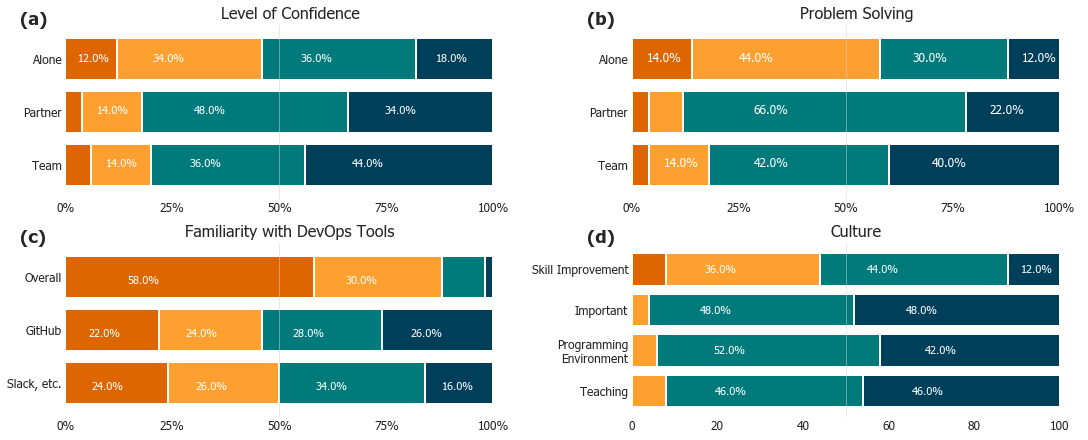
\includegraphics[width=1.9\columnwidth]{figures/Figure_Combined.png}
    \caption{Visualizations of Respondent results from Likert-Style Questions}\label{fig:likerts}
\end{figure*}

Teague et. al. \cite{teague2008collaborative} evaluated collaborative learning between novice programmers and found that it enhances their perception of programming's difficulty, their enjoyment, and their confidence. This leads to higher retention, deeper learning, and enhanced confidence when learning programming concepts. These perceptions are also influenced by different aspects such as gender, domain knowledge, experience, and stereotypes. This is supported by Tissenbaum \cite{tissenbaum2020see} when they found users shift from unproductive to productive states using the \textit{Divergent Collaboration Learning Mechanisms} (DCLM) framework. The study also found out that interactions with others played an important role in transitioning to productive states of novices. In this paper, we focus on the Philippine context as programming skills are still in high demand for both software developers and data scientists \cite{gonzales_2019, quismorio_pasquin_tayco_2020}. In this paper, we: (1) attempt to measure and assess what initial knowledge novice programmers have about DevOps. We do this investigation in reference to the \textit{Culture, Automation, Lean, Measurement, Sharing} (CALMS) model as introduced by \cite{hamunen2016challenges, riley2014keep}. We also attempt to (2) analyze the different opinions of novice programmers with regards to integrating DevOps in their processes. We do this through affinity and scenario mapping in order to discover what possible interventions we can introduce to help them in their pains and struggles. Lastly, we (3) reflect on how we can design and evaluate a tool that will support novice programmers towards adopting DevOps in their practice.

% We want to find out if they have innate practices in managing files and code versions among multiple collaborators. 

\section{Method}
The general methodology of this research follows the approach by \cite{peffers2007design} where we gathered initial user data and performed affinity analysis on the results. The process of extracting insights and deriving guidelines for novices follows the work of \cite{beyer1999contextual, holtzblatt2005rapid, good2017programming} where they investigated on novice programmers and came up with design guidelines that lead to a prototype as well. Generally, the approach involves getting insights from the users through a semi-structured approach. These will then be processed and converted into design guidelines which will unveil the needed features in the prototype. 
\subsection{Participants}
We recruited 50 undergraduate students in a computing degree program who is only starting to begin their first formal programming course in any Philippine university as participants through convenience and snowball sampling. We also considered the participants prior programming experience in their junior high school and senior high school years. We operationalized the criteria of a novice programmer based on the guidelines by \cite{teague2014longitudinal}. Each participant provided their personal details (i.e. age, sex, domicile, prior programming training) which allows for an examination of possible prior knowledge about software engineering and DevOps. We also inquired about their programming experience (both learning and practicing) and the number of years they have been programming. 
\subsection{Study Protocol and Data Analysis}
The questionnaire was sent out using an online Google Form. The questions can be found in the project website\footnote{\url{http://comet.dlsu.edu.ph/grit/questions}}. The questions were composed of a mix of Likert-style and open-ended questions that aims to (1) perform a diagnostic, measuring the initial knowledge of novice programmers regarding DevOps, (2) assess their openness towards learning DevOps and (3) record their insights on learning about DevOps. Both quantitative and qualitative answers will be processed later on to derive guidelines and insights that will be used to design an initial software prototype and its features. We wanted to investigate how open novice programmers are to the practice of DevOps and on how much they do and they do not know about it. For this, we looked into their answers in the survey and did a comparative analysis of their responses from the questions. \textit{Affinity and Scenario Mapping}. The questionnaire was developed following the CALMS model by \cite{riley2014keep} and were organized based on each of the factors described and the Likert-style questions are measured using 4 levels: 1 - strongly disagree (dark orange), 2 - disagree (light orange), 3 - agree (light green), and 4 - strongly agree (dark green). Some of the questions required qualitative insights in the form of essays and long texts which need to be analyzed properly. We used an affinity map to categorize the different types of support needed. %pink qualitative answers. 
We grouped their insights into three color codes for easy referencing: pink for the support category, yellow for the sample support insight, and blue for an implementation idea for the prototype. From the affinity map, we derived five types of support categories that the respondents needed. These categories will serve as the design guidelines that may potentially support the affordances of our novice programmers. They are: (1) Language Specific Support, (2) Communication Specific Support, (3) Mentorship Support, (4) Process (How to) DevOps Support, and (5) Personal Support. The insights from the affinity map were converted to a scenario map and came up with one initial prototype. 

% This was followed by a scenario mapping session where we brainstormed on features from existing DevOps tools and other features that can be augmented to provide novice support based on the guidelines. %See Fig.\ref{fig:Affinity} for the affinity and scenario map used. 

% We applied affinity mapping\cite{lucero2015using} on these insights to be able to sort and rank the problems that we can identify to ultimately support that prototype that is described in the latter part of this paper. From this, we derived ideas and compared these with existing DevOps tools. After a brainstorming and mapping session, we designed features into a high fidelity mock-up that will be tested and evaluated iteratively by its target users. 
\begin{comment}
\begin{figure*}[tp]
    \centering
    \includegraphics[width=1.75\columnwidth]{"figures/DevOpsX Qualitative Affinity for Prototype Design"}
    \caption{Affinity Map and Scenario Map containing insights and ideas for \texit{Grit}}
    \label{fig:Affinity}
\end{figure*}
\end{comment}
\section{Results and Findings}
The inidividual results can be found as listed in our project website\footnote{\url{http://comet.dlsu.edu.ph/grit/results}}.  Based on Fig.\ref{fig:likerts}(a), more than half of the respondents are confident in working regardless of whether they are alone, with a partner, or with a team. However, most respondents prefer having more people to work with than having to work alone.  In contrast to this, the confidence levels of novice programmers plummet when asked about their capabilities in problem-solving. As seen in Fig.\ref{fig:likerts}(b), 54\% find it more difficult to solve problems when working alone. Concerning this, majority of the respondents find it easier to work with teammates. From the study we also looked at the familiarity of novice programmers with the different DevOps Tools as seen in Fig.\ref{fig:likerts}(c). Majority (58\%) are not familiar with the various DevOps tools in general. However, more than half were familiar with GitHub though it is believed that not all who are not familiar with DevOps tools may be familiar with Github as a DevOps tool. Moreover, it can be hypothesized that people still opt to do face-to-face communication than to use communication/social applications. The results also show that half of the respondents use professional communication software such as \textit{Slack}, \textit{Google Hangouts}, etc. If we wish to further analyze the corresponding DevOps culture in Fig.\ref{fig:likerts}(d), we can see that novice programmers think that DevOps is important (96\%) and should be taught in school (92\%). However, on the question of whether it is important to learn DevOps to become better in programming, almost half (44\%) were unsure whether it was relevant to become a better developer. With regards to the collaboration culture of DevOps, we observe that majority of the respondents (57.4\%) strongly perceived it as a platform for knowledge sharing and trust \& respect. This is an interesting take as it sparks the discussion that even as novices, they understand wholly that trust and respect are key elements in collaborative activities such as DevOps. Additionally, the respondents perceived DevOps as a collaborative process that involves pair programming and working in teams. Looking back at Fig.\ref{fig:likerts}(a), we observed that there was a distinct decrease in confidence of the respondents when compared to the general level of confidence in problem-solving scenarios. Moreover, we noticed that most respondents prefer having more people to work with, than being entirely alone. There is an obvious decrease in respondents agreeing about their confidence in working with others as compared to working alone.
\section{Discussion}
% For the purpose of collecting results, we have arbitrarily chosen the responses under Culture, Automation and Sharing only since (1) these are aligned with the objective of assessing the openness and initial knowledge of novice programmers and (2) these factors are not observed unlike Lean and Measurement factors as seen in the work of \cite{fronza2011understanding}.
% We used an affinity map to categorize the different types of support needed. %pink qualitative answers. 
% We grouped their insights into three color codes for easy referencing: pink for the support category, yellow for the sample support insight, and blue for an implementation idea for the prototype. From the affinity map, we derived five types of support categories that the respondents needed. These categories will serve as the design guidelines that may potentially support the affordances of our novice programmers. They are: (1) Language Specific Support, (2) Communication Specific Support, (3) Mentorship Support, (4) Process (How to) DevOps Support, and (5) Personal Support. This was followed by a scenario mapping session where we brainstormed on features from existing DevOps tools and other features that can be augmented to provide novice support based on the guidelines. %See Fig.\ref{fig:Affinity} for the affinity and scenario map used. 
\subsection{Proposed Prototype Features}
Upon analyzing the data gathered, we designed a prototype that is intended to help novice programmers in integrating DevOps in their projects and processes. We call this proposed system as \textit{Grit}, which shall serve as a platform to guide novice programmers starting with DevOps. It will have the regular features from Git but will be augmented with six main features namely: (1) \textit{Version Control module}, (2) Virtual Assistant, (3) Command-Line with Predictive Text, (4) Coachmarks, (5) Practice with Codeblocks and a feature accessed only online called (6) Find-a-Coach. Fig.\ref{fig:mockup} shows a mock-up of these features. More details as well as a closer look on the mockups can be found in our project website\footnote{\url{http://comet.dlsu.edu.ph/grit/screenshots}}. The \textit{version control module} is based on GitHub desktop which can run git commands such as pull, push, and commit. The Virtual Assistant serves as a guided walkthrough for the git commands and its functions. Additionally, the Command-Line feature allows the users to call git commands with predictive text. Likewise, the Coachmark enables first time users to navigate through the system easily. On the other hand, the practice with Codeblocks feature helps users to practice and understand the basic git commands. Lastly, the Find-a-Coach feature is an online mentoring tool that allows novices to find a mentor that will guide them through their DevOps process real-time. With these proposed features, we seek to investigate whether these novices can be accustomed to the DevOps process but these would still have to be verified through further tests and experiments. 
\begin{comment}
\begin{figure}[tp]
    \centering
    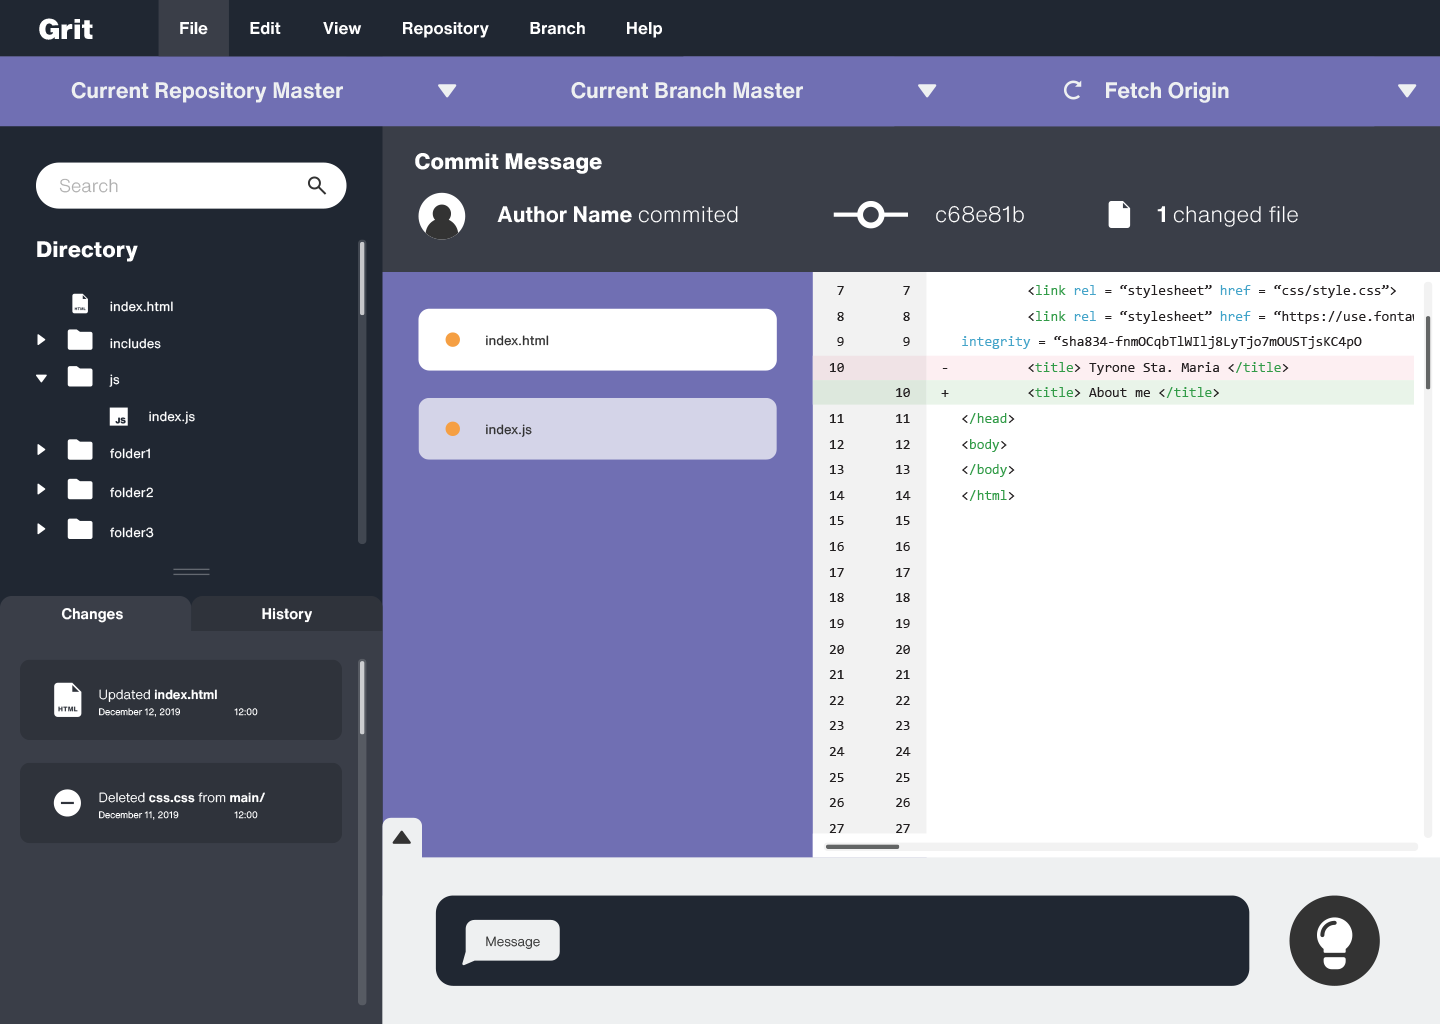
\includegraphics[width=1\columnwidth]{figures/mockup1}
    \caption{Preview of \textit{Grit} and some of its features}
    \label{fig:mockup}
\end{figure}
\end{comment}
\section{Conclusion and Future Work}
In this study, we were able provide an initial understanding on the readiness of novice programmers to do DevOps. The collected data still needs further analysis. We were able to inquire into their insights considering the \textit{Culture, Automation} and \textit{Sharing} aspects of the CALMS model. We synthesized and extracted these insights into factors that may potentially support affordances of novice programmers in integrating DevOps in their practice. This allowed us to initially understand their pains and struggles but this is still subject to further inquiry and validation. Lastly, we were able to create a mock-up design of \textit{Grit} to augment Novice DevOps experiences. Since the study focused on novices, we believe it would be an interesting approach to gather and understand the insights of adept and more experienced programmers as well. This way, we could do a retrospective approach on the pains and struggles that we intend to investigate. The same focus can also be done on expert DevOps practitioners. The study can take another approach in inquiring into their perceived effectiveness, level of engagement, and other factors that can be attributed to their readiness to do DevOps. A participatory study can also be done to review and evaluate the proposed features of Grit. Since DevOps involves Software Industry practices, we can also do an investigation and cross-comparison of novice programmer insights with experienced industry practitioners with the help of the \textit{Functionality, Usability, Supportability, Reliability, Performance} (FURPS) model in practice \cite{al2010quality}.
The study mainly focused on the novice programmers' familiarity of DevOps practices and tools such as git and github, we believe that we should also take into account the respondents' familiarity with core DevOps tools like build servers or deployment platforms. This can help us assess their knowledge and improve Grit's features. 
\balance{}
\bibliographystyle{SIGCHI-Reference-Format}
\bibliography{myreferences}
\end{document}